\documentclass[11pt]{article}

\usepackage[utf8]{inputenc}
\usepackage[T1]{fontenc}
\usepackage{geometry}
\geometry{a4paper, margin=2.5cm}
\usepackage{graphicx}
\usepackage{booktabs}
\usepackage{multirow}
\usepackage{hyperref}
\usepackage{xcolor}
\usepackage{longtable}
\usepackage{float}
\usepackage{caption}
\usepackage{subcaption}

\hypersetup{
    colorlinks=true,
    linkcolor=blue!70!black,
    citecolor=blue!70!black,
    urlcolor=blue!70!black
}

\title{\textbf{Supplementary Information}\\[0.5em]
\large hvantk: a Hail-based toolkit for scalable variant annotation, multi-omics integration, and downstream enrichment analysis}

\author{Enrique Audain, Yasset Perez-Riverol, Marc-Phillip Hitz}

\date{}

\begin{document}

\maketitle

\tableofcontents
\newpage

%============================================================================
% PSROC RESULTS
%============================================================================
\section{PSROC Module: Prediction Score ROC Analysis}

To demonstrate the PSROC module, we evaluated three pathogenicity prediction scores (CADD, REVEL, and MetaLR) using a synthetic dataset of 100 variants from cancer-associated genes (BRCA1, BRCA2, TP53). After excluding variants with uncertain significance, 90 variants (50 pathogenic, 40 benign) were used for ROC analysis.

\subsection{ROC Curve Analysis}

Figure~\ref{fig:roc_curves} shows the receiver operating characteristic (ROC) curves for each prediction score. REVEL achieved the highest discriminative performance (AUC = 0.998), followed by CADD (AUC = 0.979) and MetaLR (AUC = 0.896).

\begin{figure}[H]
    \centering
    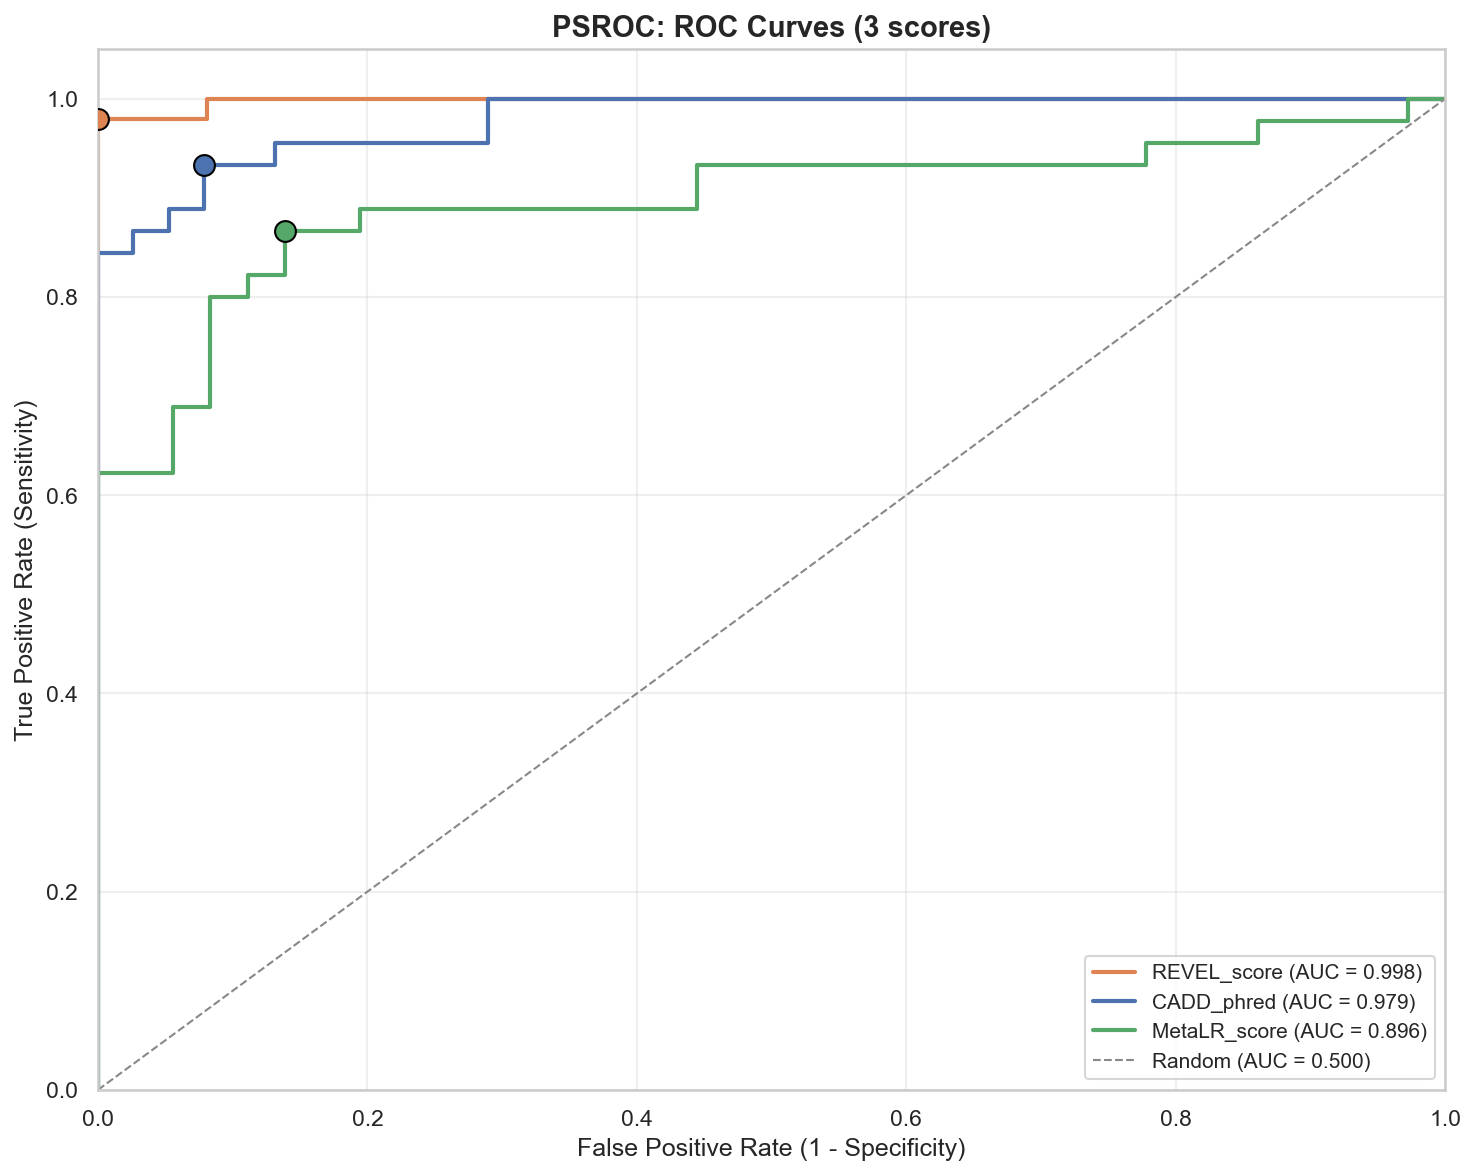
\includegraphics[width=0.85\textwidth]{figures/fig_s1_roc_curves.png}
    \caption{\textbf{ROC curves for pathogenicity prediction scores.} Performance comparison of CADD, REVEL, and MetaLR scores for discriminating pathogenic from benign variants in BRCA1, BRCA2, and TP53. The diagonal dashed line represents random classification (AUC = 0.5).}
    \label{fig:roc_curves}
\end{figure}

\subsection{Performance Metrics}

Table~\ref{tab:psroc_metrics} summarizes the performance metrics for each prediction score, including AUC, optimal classification thresholds (determined by Youden's J statistic), and sensitivity/specificity at the optimal threshold.

\begin{table}[H]
\centering
\caption{\textbf{PSROC performance metrics for pathogenicity prediction scores.}}
\label{tab:psroc_metrics}
\begin{tabular}{@{}lccccc@{}}
\toprule
\textbf{Score} & \textbf{AUC} & \textbf{Optimal Threshold} & \textbf{Sensitivity} & \textbf{Specificity} & \textbf{Missingness} \\
\midrule
REVEL & 0.998 & 0.454 & 0.980 & 1.000 & 3.3\% \\
CADD (phred) & 0.979 & 16.42 & 0.933 & 0.921 & 7.8\% \\
MetaLR & 0.896 & 0.500 & 0.867 & 0.861 & 10.0\% \\
\bottomrule
\end{tabular}
\end{table}

\subsection{AUC Comparison}

Figure~\ref{fig:auc_comparison} provides a visual comparison of AUC values across the three prediction scores, highlighting REVEL's superior performance in this example dataset.

\begin{figure}[H]
    \centering
    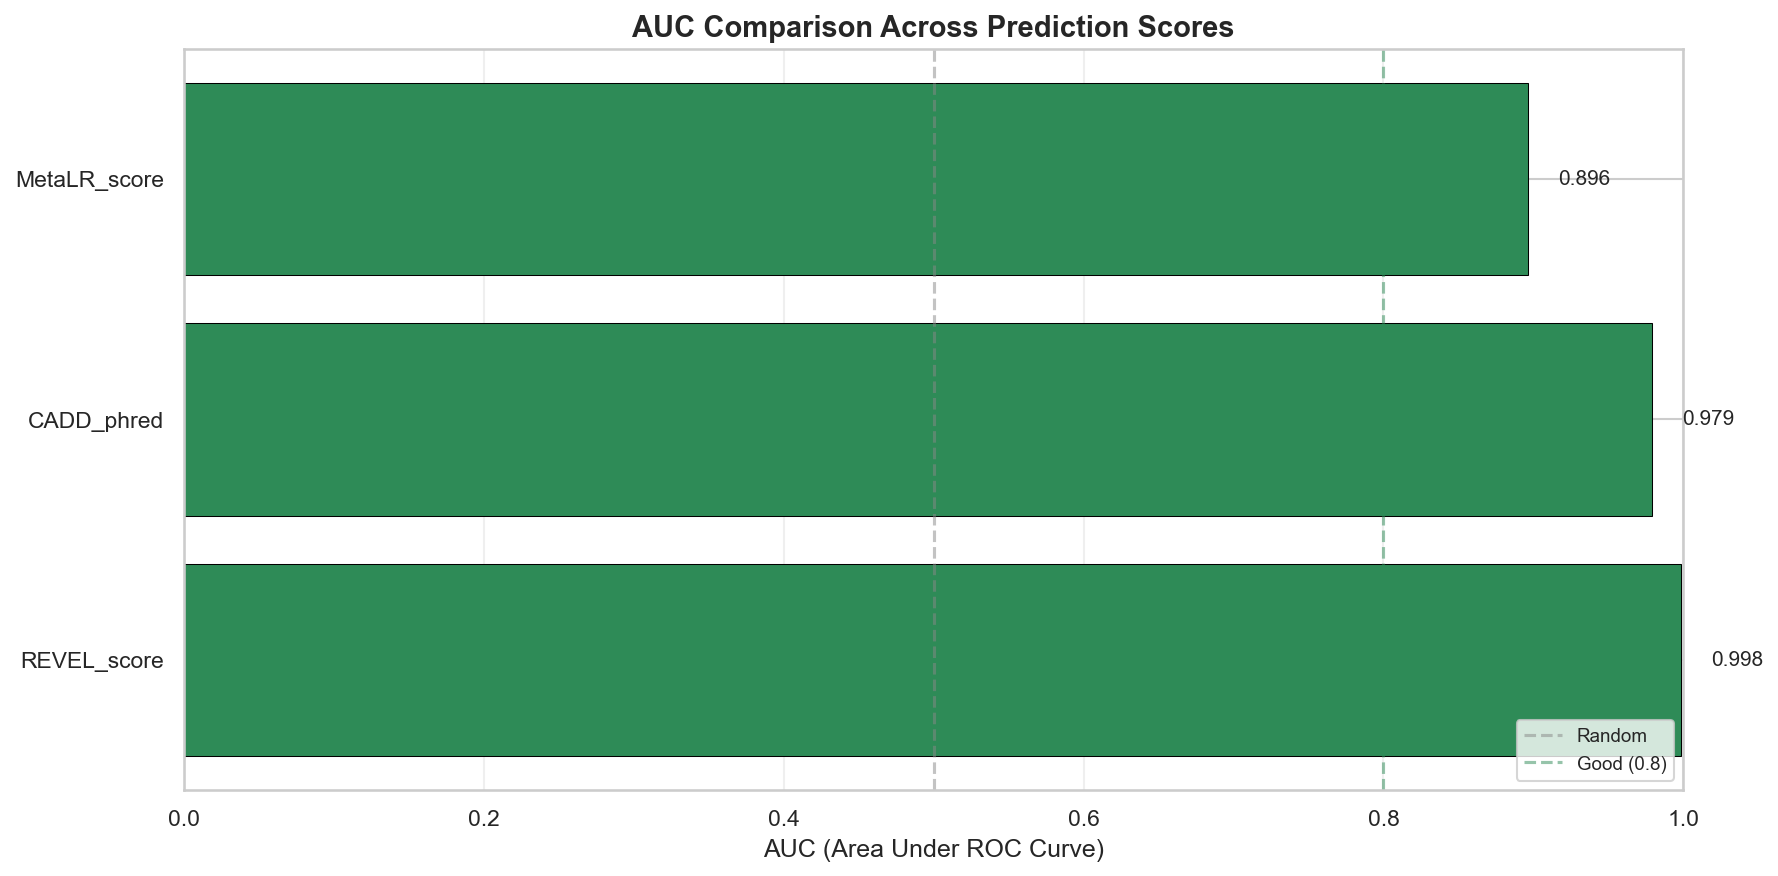
\includegraphics[width=0.7\textwidth]{figures/fig_s2_auc_comparison.png}
    \caption{\textbf{AUC comparison across prediction scores.} Bar chart comparing area under the ROC curve for CADD, REVEL, and MetaLR pathogenicity prediction scores.}
    \label{fig:auc_comparison}
\end{figure}

\newpage
%============================================================================
% ENRICHEX OVERLAP RESULTS
%============================================================================
\section{EnrichEx Module: Overlap Enrichment Analysis}

The overlap enrichment analysis tests whether a query gene list is significantly enriched in predefined gene sets using Fisher's exact test. We demonstrate this functionality using a set of Alzheimer's disease-associated genes tested against brain cell-type-specific gene sets.

\subsection{Overlap Enrichment Results}

Table~\ref{tab:overlap_results} shows the overlap enrichment results for 8 query genes tested against 6 brain cell-type gene sets (35 background genes). The analysis identifies potential cell-type-specific enrichment patterns.

\begin{table}[H]
\centering
\caption{\textbf{Overlap enrichment results for brain cell-type gene sets.} Fisher's exact test results showing odds ratios, p-values, and Benjamini-Hochberg adjusted p-values.}
\label{tab:overlap_results}
\begin{tabular}{@{}lccccc@{}}
\toprule
\textbf{Gene Set} & \textbf{n Overlap} & \textbf{Odds Ratio} & \textbf{95\% CI} & \textbf{P-value} & \textbf{P-adj} \\
\midrule
Excitatory Neurons & 2 & 7.96 & 0.36--528.0 & 0.124 & 0.744 \\
Microglia & 4 & 2.31 & 0.34--16.0 & 0.402 & 0.805 \\
Astrocytes & 2 & 1.16 & 0.09--9.2 & 1.000 & 1.000 \\
Oligodendrocytes & 0 & 0.00 & 0.00--3.8 & 0.315 & 0.805 \\
Endothelial & 0 & 0.00 & 0.00--5.3 & 0.553 & 0.830 \\
Inhibitory Neurons & 0 & 0.00 & 0.00--8.5 & 1.000 & 1.000 \\
\bottomrule
\end{tabular}
\end{table}

\subsection{Overlap Enrichment Visualization}

Figure~\ref{fig:overlap_enrichment} shows a dot plot visualization of the overlap enrichment results, with dot size representing the number of overlapping genes and color indicating statistical significance.

\begin{figure}[H]
    \centering
    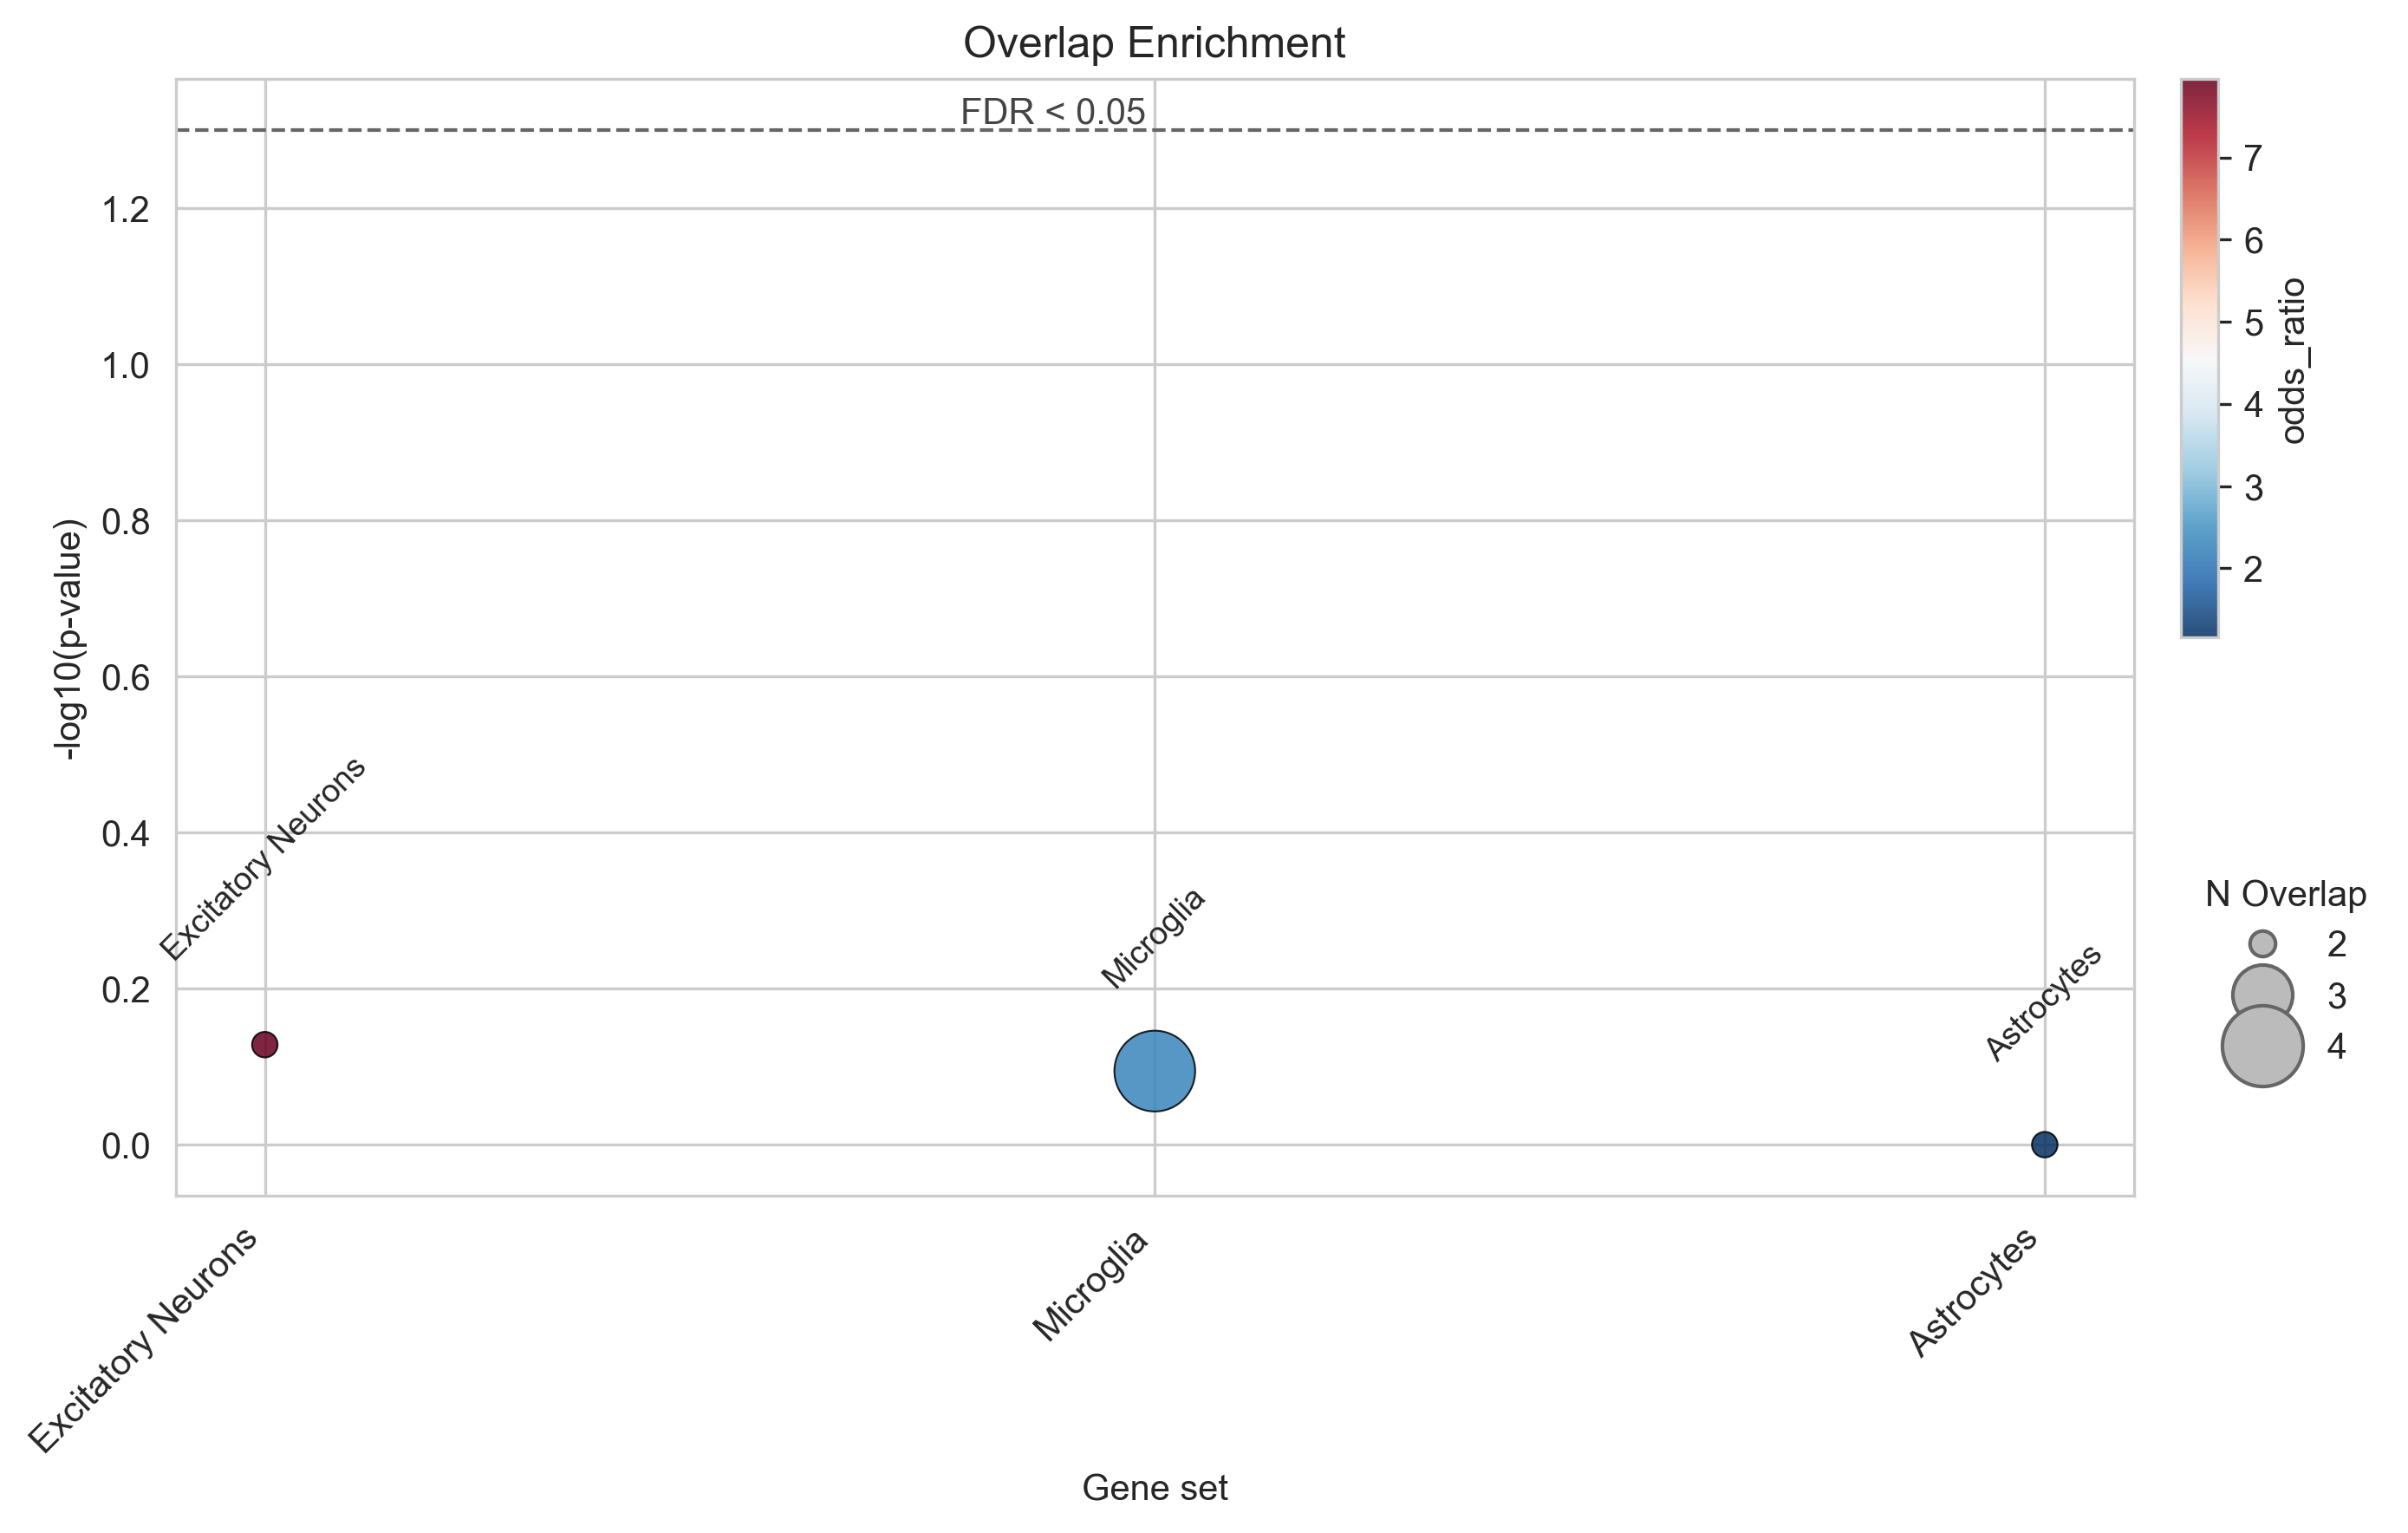
\includegraphics[width=0.85\textwidth]{figures/fig_s3_overlap_enrichment.png}
    \caption{\textbf{Overlap enrichment dot plot.} Gene set enrichment results showing -log10(p-value) on the x-axis. Dot size corresponds to the number of overlapping genes between the query set and each gene set. Color indicates odds ratio magnitude.}
    \label{fig:overlap_enrichment}
\end{figure}

\newpage
%============================================================================
% ENRICHEX BURDEN RESULTS
%============================================================================
\section{EnrichEx Module: Rare Variant Burden Testing}

The burden testing module evaluates whether rare variant burden in gene sets is associated with phenotypes using Hail's regression framework. We demonstrate this using logistic regression to test associations between rare variant burden and a binary phenotype across brain cell-type gene sets.

\subsection{Burden Testing Results}

Table~\ref{tab:burden_results} shows the logistic regression results for rare variant burden analysis. Effect sizes (beta coefficients), odds ratios with 95\% confidence intervals, and p-values are reported for each gene set.

\begin{table}[H]
\centering
\caption{\textbf{Rare variant burden testing results.} Logistic regression analysis of rare variant burden association with phenotype across brain cell-type gene sets.}
\label{tab:burden_results}
\begin{tabular}{@{}lcccccc@{}}
\toprule
\textbf{Gene Set} & \textbf{Beta} & \textbf{SE} & \textbf{OR} & \textbf{95\% CI} & \textbf{P-value} & \textbf{P-adj} \\
\midrule
Excitatory Neurons & 0.539 & 0.613 & 1.71 & 0.52--5.70 & 0.379 & 0.568 \\
Astrocytes & 0.511 & 0.379 & 1.67 & 0.79--3.50 & 0.177 & 0.524 \\
Microglia & 0.298 & 0.266 & 1.35 & 0.80--2.27 & 0.262 & 0.524 \\
Endothelial & 0.000 & 0.393 & 1.00 & 0.46--2.16 & 1.000 & 1.000 \\
Oligodendrocytes & -0.288 & 0.760 & 0.75 & 0.17--3.33 & 0.705 & 0.846 \\
Inhibitory Neurons & -0.731 & 0.632 & 0.48 & 0.14--1.66 & 0.248 & 0.524 \\
\bottomrule
\end{tabular}
\end{table}

\subsection{Burden Testing Forest Plot}

Figure~\ref{fig:burden_forest} shows a forest plot of the burden testing results, displaying odds ratios with 95\% confidence intervals for each gene set.

\begin{figure}[H]
    \centering
    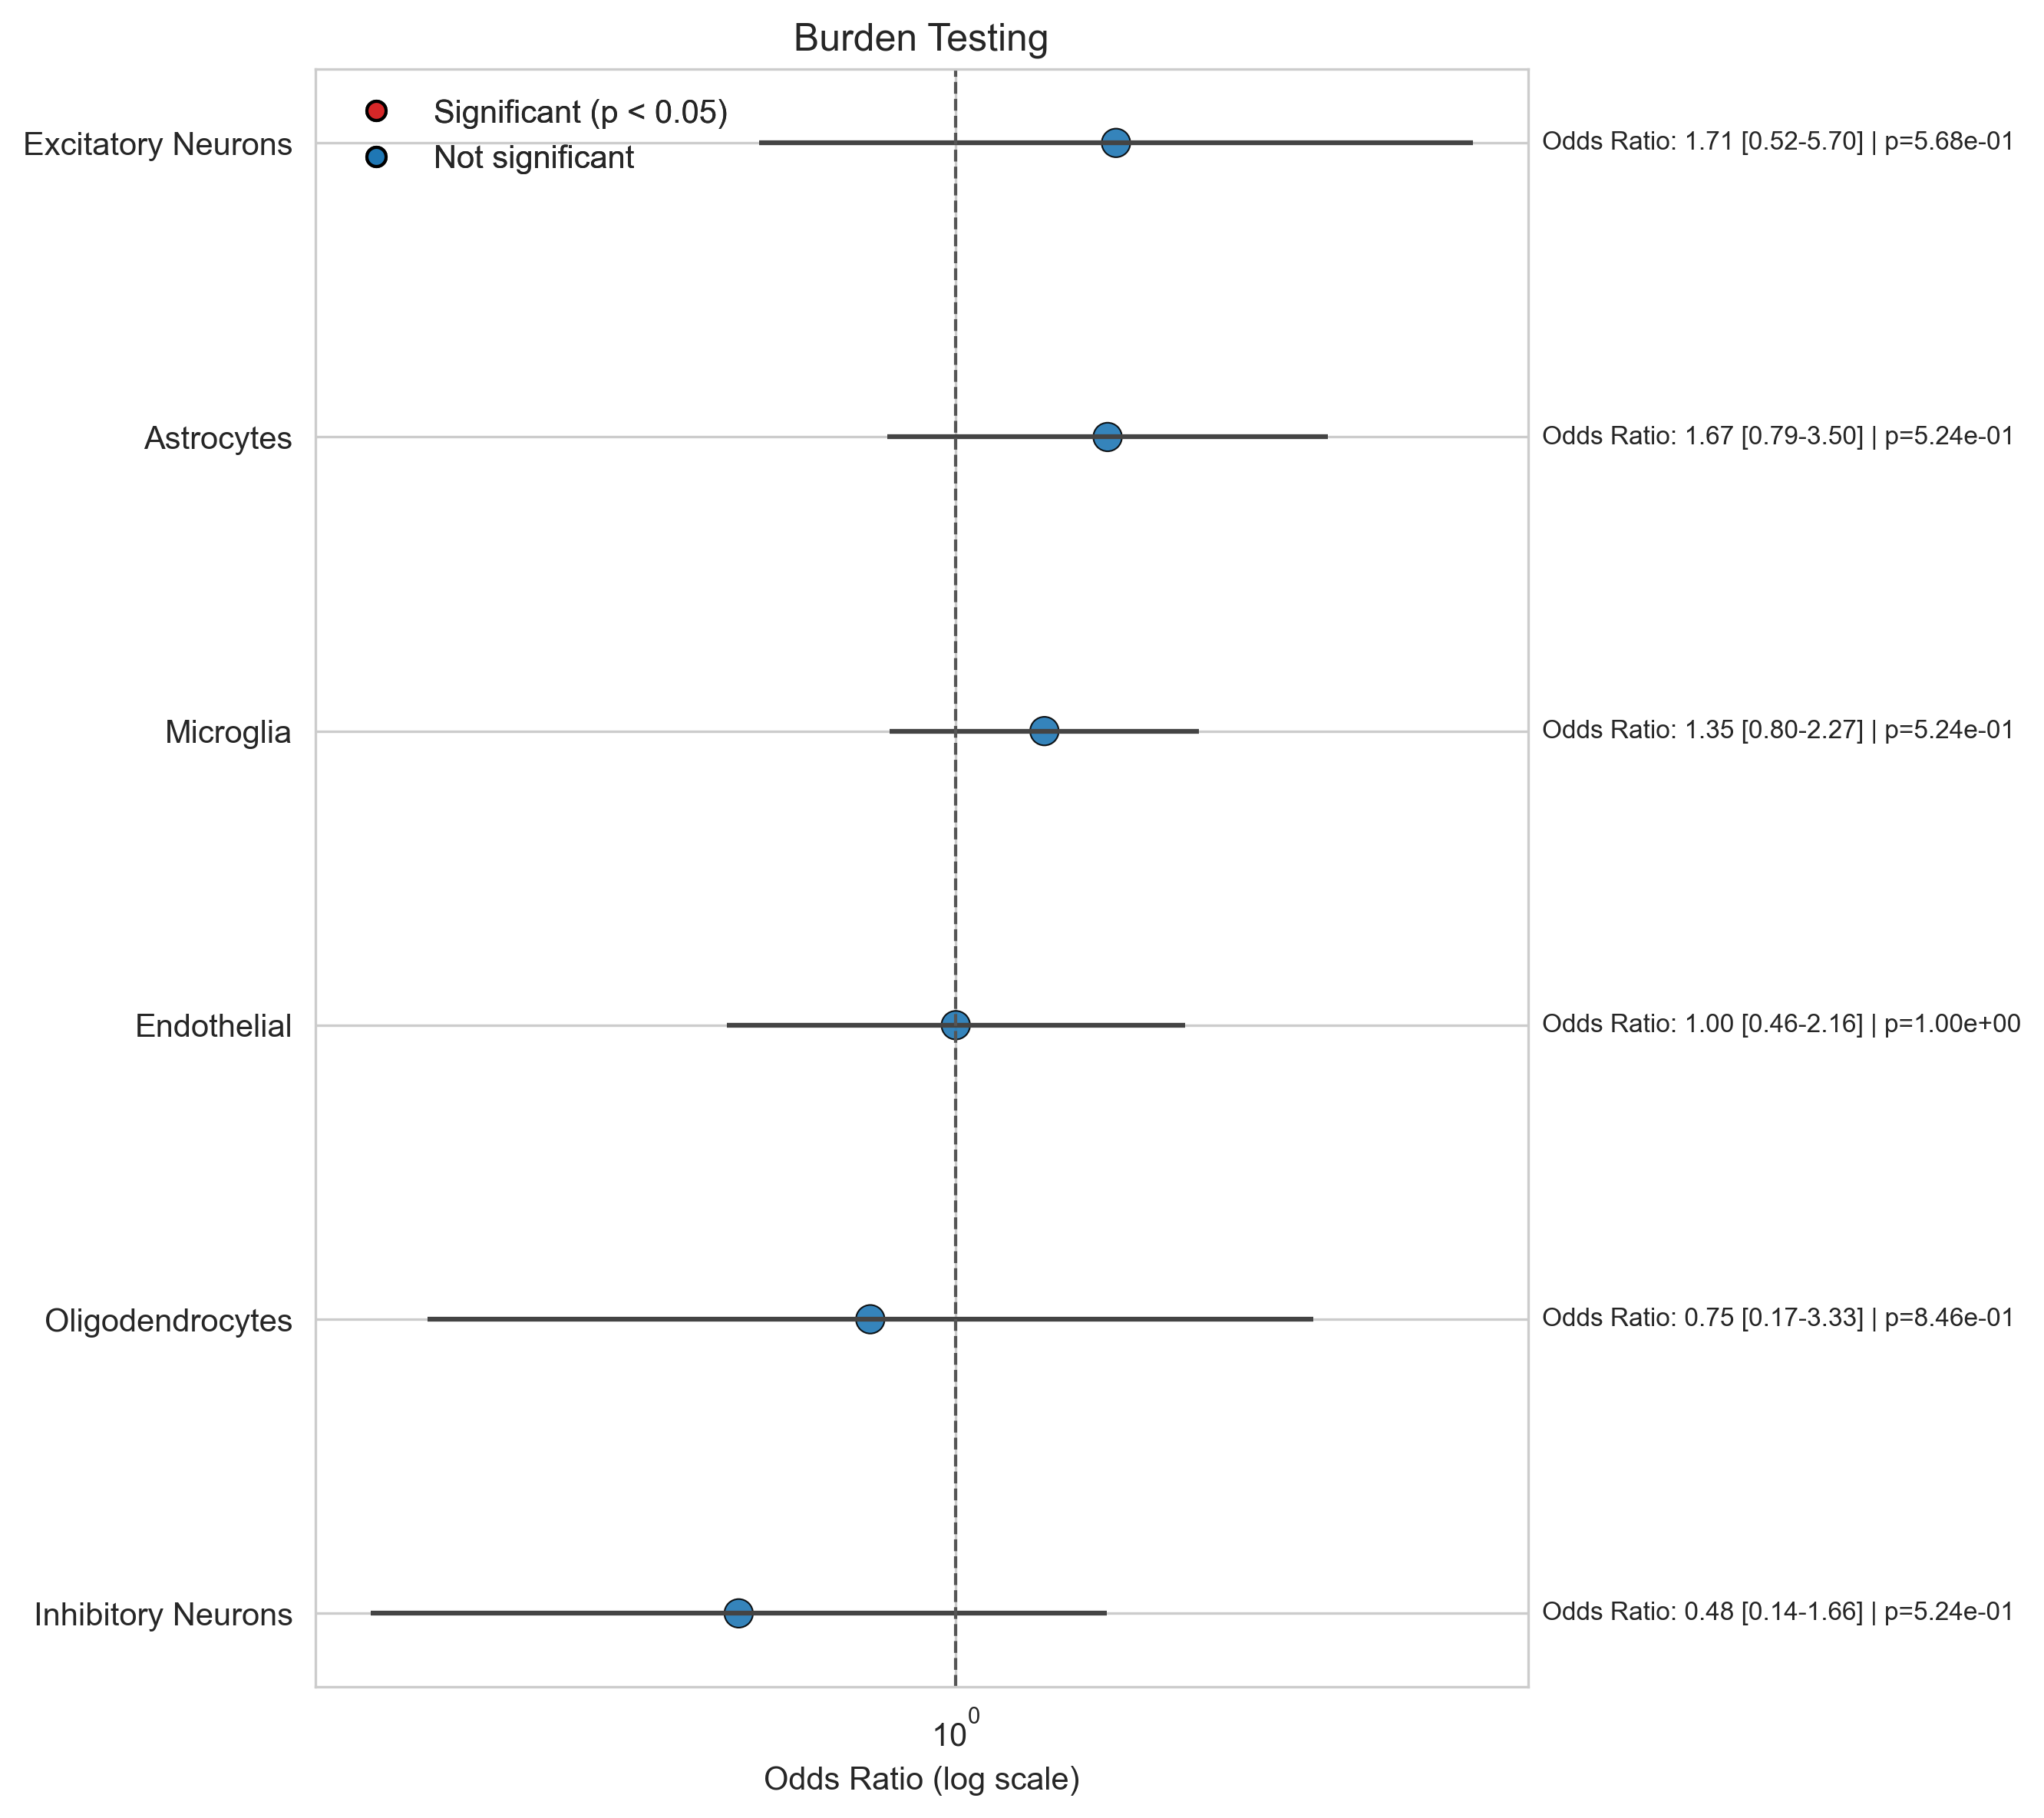
\includegraphics[width=0.85\textwidth]{figures/fig_s4_burden_forest.png}
    \caption{\textbf{Burden testing forest plot.} Odds ratios with 95\% confidence intervals from logistic regression analysis of rare variant burden. The vertical dashed line at OR = 1 indicates no association. Gene sets are ordered by effect size.}
    \label{fig:burden_forest}
\end{figure}

\newpage
%============================================================================
% HGC QC RESULTS
%============================================================================
\section{Quality Control Reporting}

hvantk provides integrated quality control reporting for VDS-derived MatrixTables. The QC module computes sample-level and variant-level metrics and generates interactive HTML reports with publication-ready visualizations.

\subsection{QC Dashboard}

Figure~\ref{fig:qc_dashboard} shows an example QC dashboard generated by hvantk, including sample call rates, heterozygosity distributions, transition/transversion ratios, and variant quality metrics.

\begin{figure}[H]
    \centering
    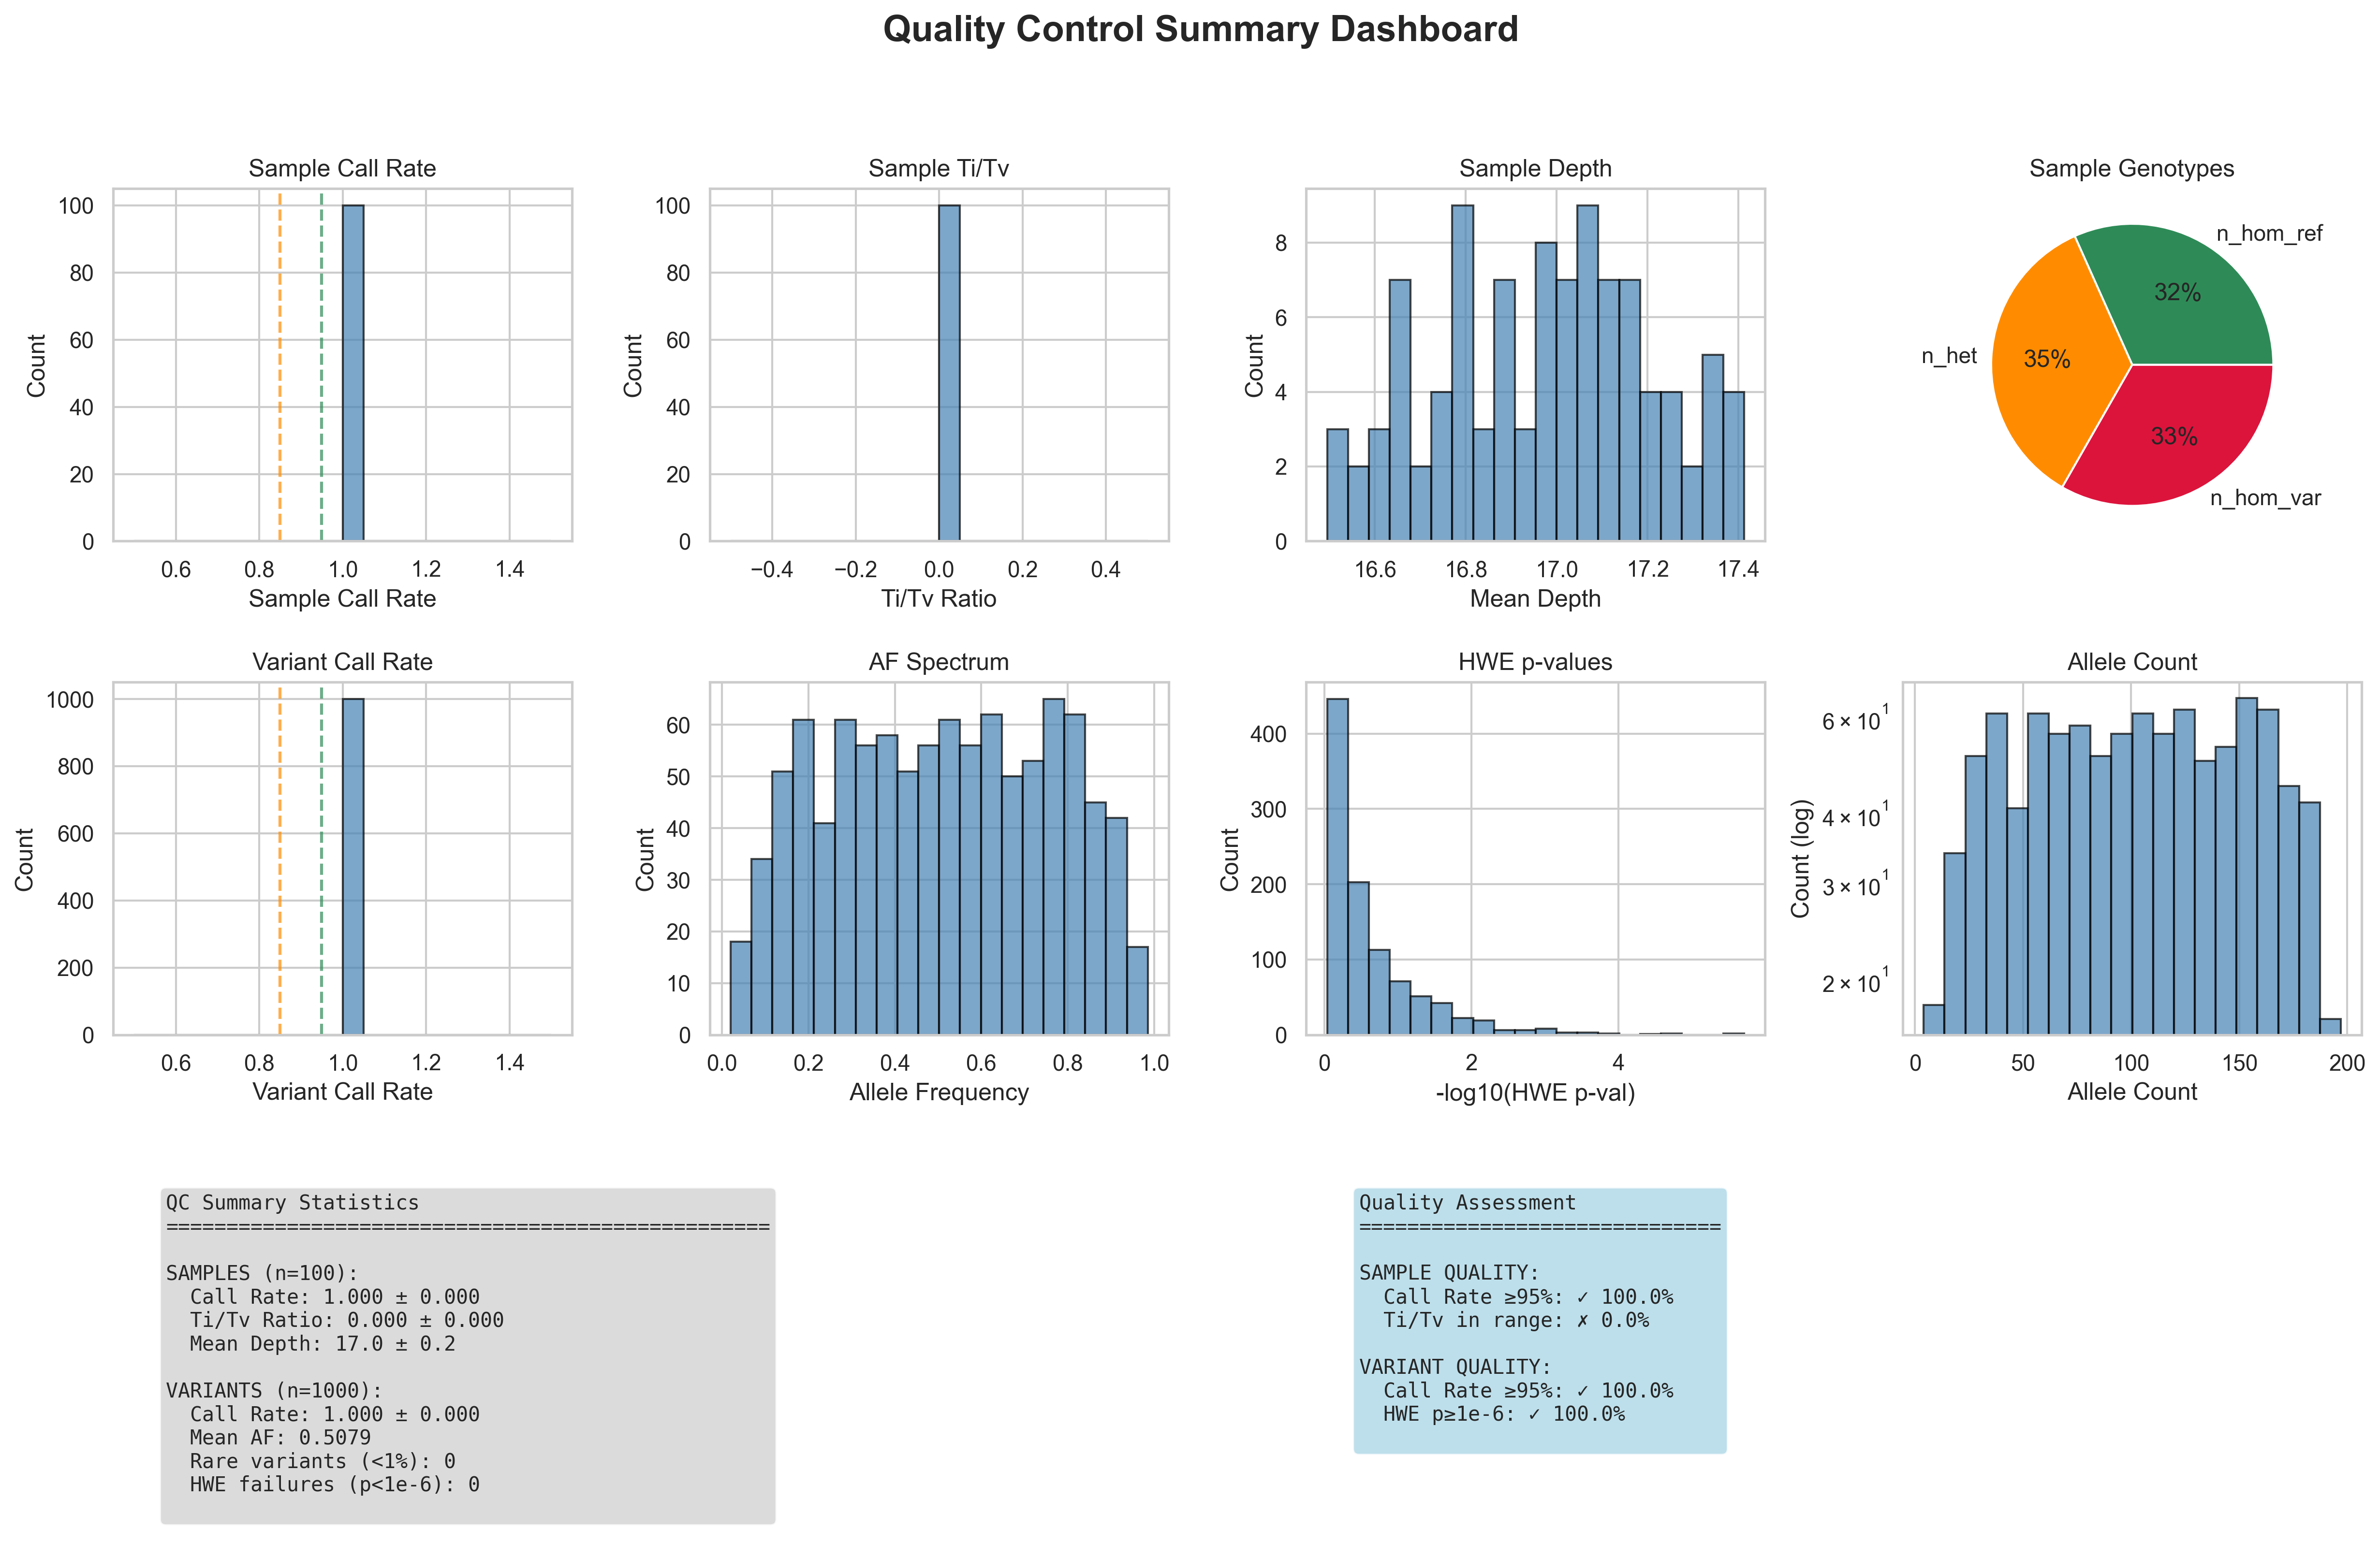
\includegraphics[width=\textwidth]{figures/fig_s5_qc_dashboard.png}
    \caption{\textbf{Quality control dashboard.} Multi-panel visualization showing sample-level QC metrics including call rate distribution, heterozygosity, Ti/Tv ratio, and variant-level statistics. This dashboard is automatically generated by the \texttt{hvantk hgc qc-report} command.}
    \label{fig:qc_dashboard}
\end{figure}

\newpage
%============================================================================
% PERFORMANCE BENCHMARKS
%============================================================================
\section{Performance Benchmarks}

To evaluate hvantk's scalability, we conducted CPU scaling benchmarks measuring execution time across different computational configurations.

\subsection{CPU Scaling Analysis}

Figure~\ref{fig:cpu_scaling} shows the breakdown of execution time by workflow step across different CPU configurations, demonstrating the toolkit's ability to leverage parallel processing for computationally intensive operations.

\begin{figure}[H]
    \centering
    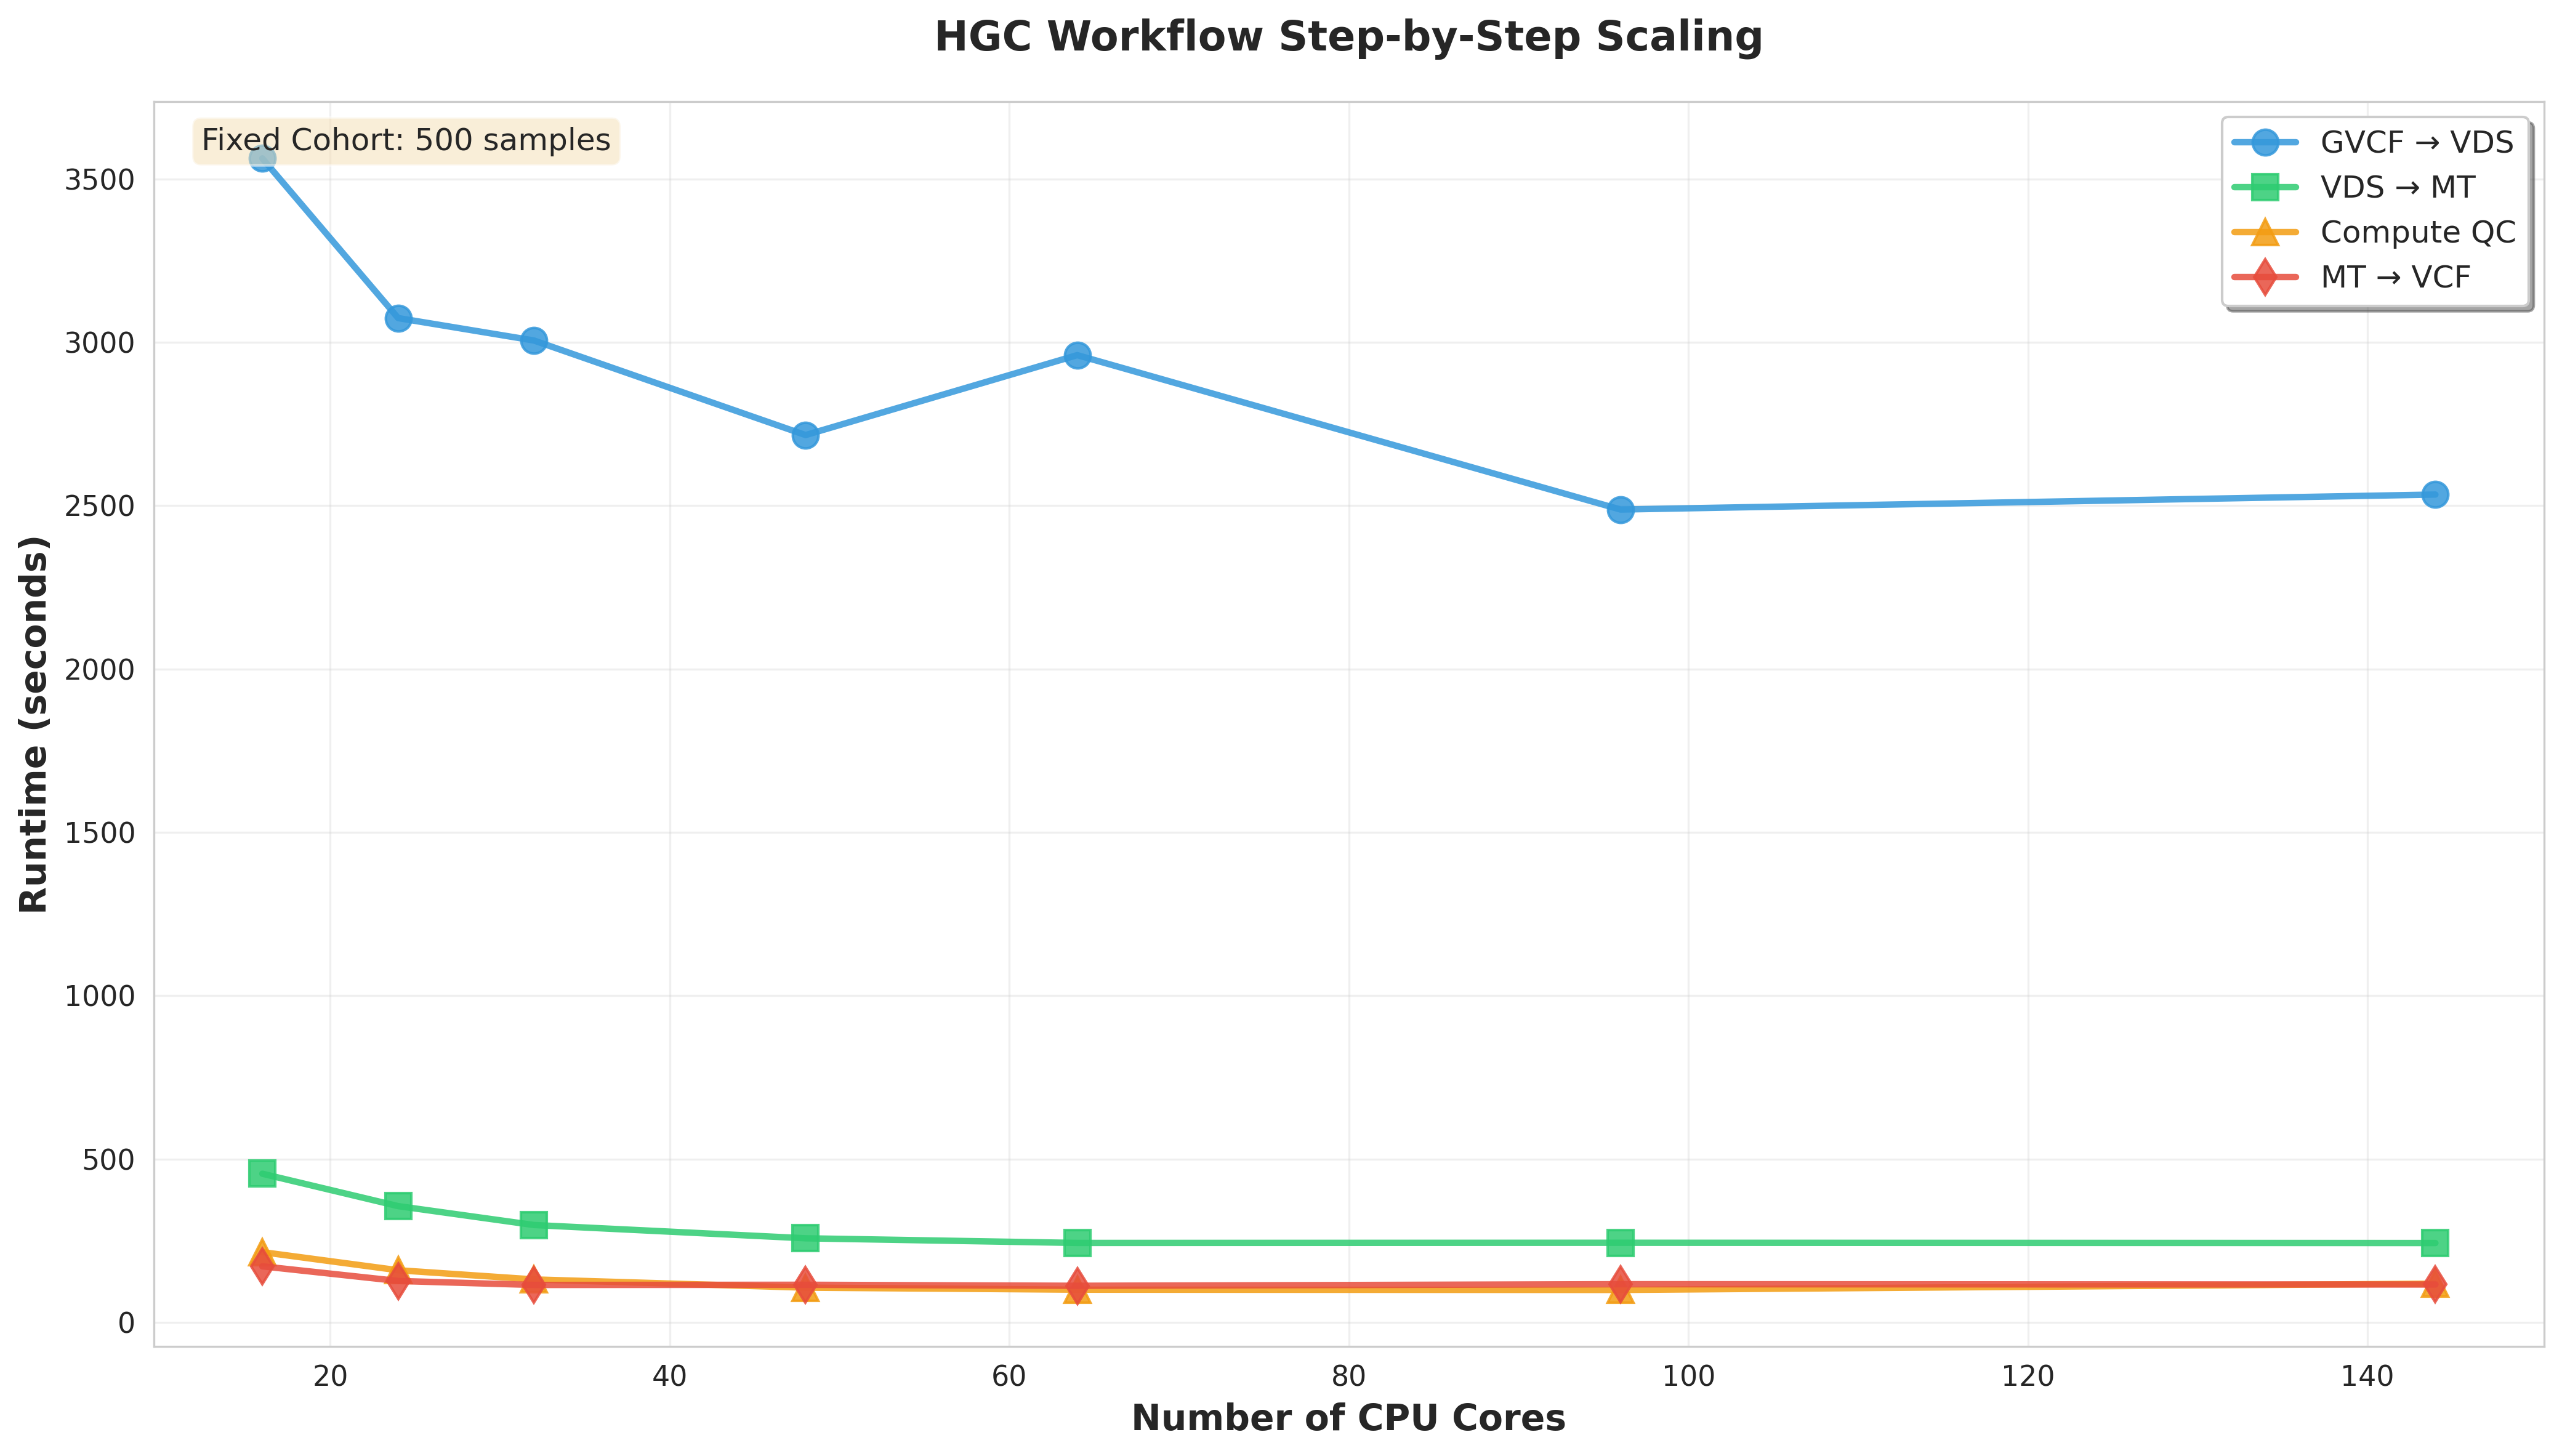
\includegraphics[width=0.9\textwidth]{figures/fig_s6_cpu_scaling.png}
    \caption{\textbf{CPU scaling performance analysis.} Breakdown of execution time by workflow step (GVCF combination, VDS conversion, QC computation) across different CPU configurations. Results demonstrate strong scaling behavior for parallelizable operations.}
    \label{fig:cpu_scaling}
\end{figure}

\newpage
%============================================================================
% DATA AVAILABILITY
%============================================================================
\section{Data and Code Availability}

All example scripts and synthetic datasets used to generate the results in this supplementary information are available in the hvantk repository:

\begin{itemize}
    \item \textbf{PSROC example}: \texttt{examples/psroc/run\_psroc\_example.py}
    \item \textbf{EnrichEx overlap}: \texttt{examples/enrichex/overlap\_enrichment\_example.py}
    \item \textbf{EnrichEx burden}: \texttt{examples/enrichex/burden\_analysis\_example.py}
    \item \textbf{HGC QC example}: \texttt{examples/hgc/hgc\_qc\_example.py}
    \item \textbf{Benchmark scripts}: \texttt{examples/hgc/scripts/}
\end{itemize}

Interactive HTML reports with additional details are generated by each workflow and can be found in the respective \texttt{results/} directories.

\end{document}
